\documentclass[aspectratio=169,professionalfonts]{beamer}

\usepackage[T1]{fontenc}
\usepackage{helvet}
\usepackage[main=english]{babel}
\usepackage{amssymb,amsmath,amsfonts,amsthm}
\usepackage[style=american]{csquotes}
\usepackage{multicol}
%\usepackage{enumitem}

\beamertemplatenavigationsymbolsempty
\renewcommand{\familydefault}{\sfdefault}
\setbeamercolor{block title}{bg=red!30,fg=black}
\setbeamercolor{block body}{fg=black,bg=gray!10}
\setbeamercolor{block body example}{fg=black,bg=gray!10}
\setbeamertemplate{blocks}[rounded][shadow=false]

\usebackgroundtemplate{%
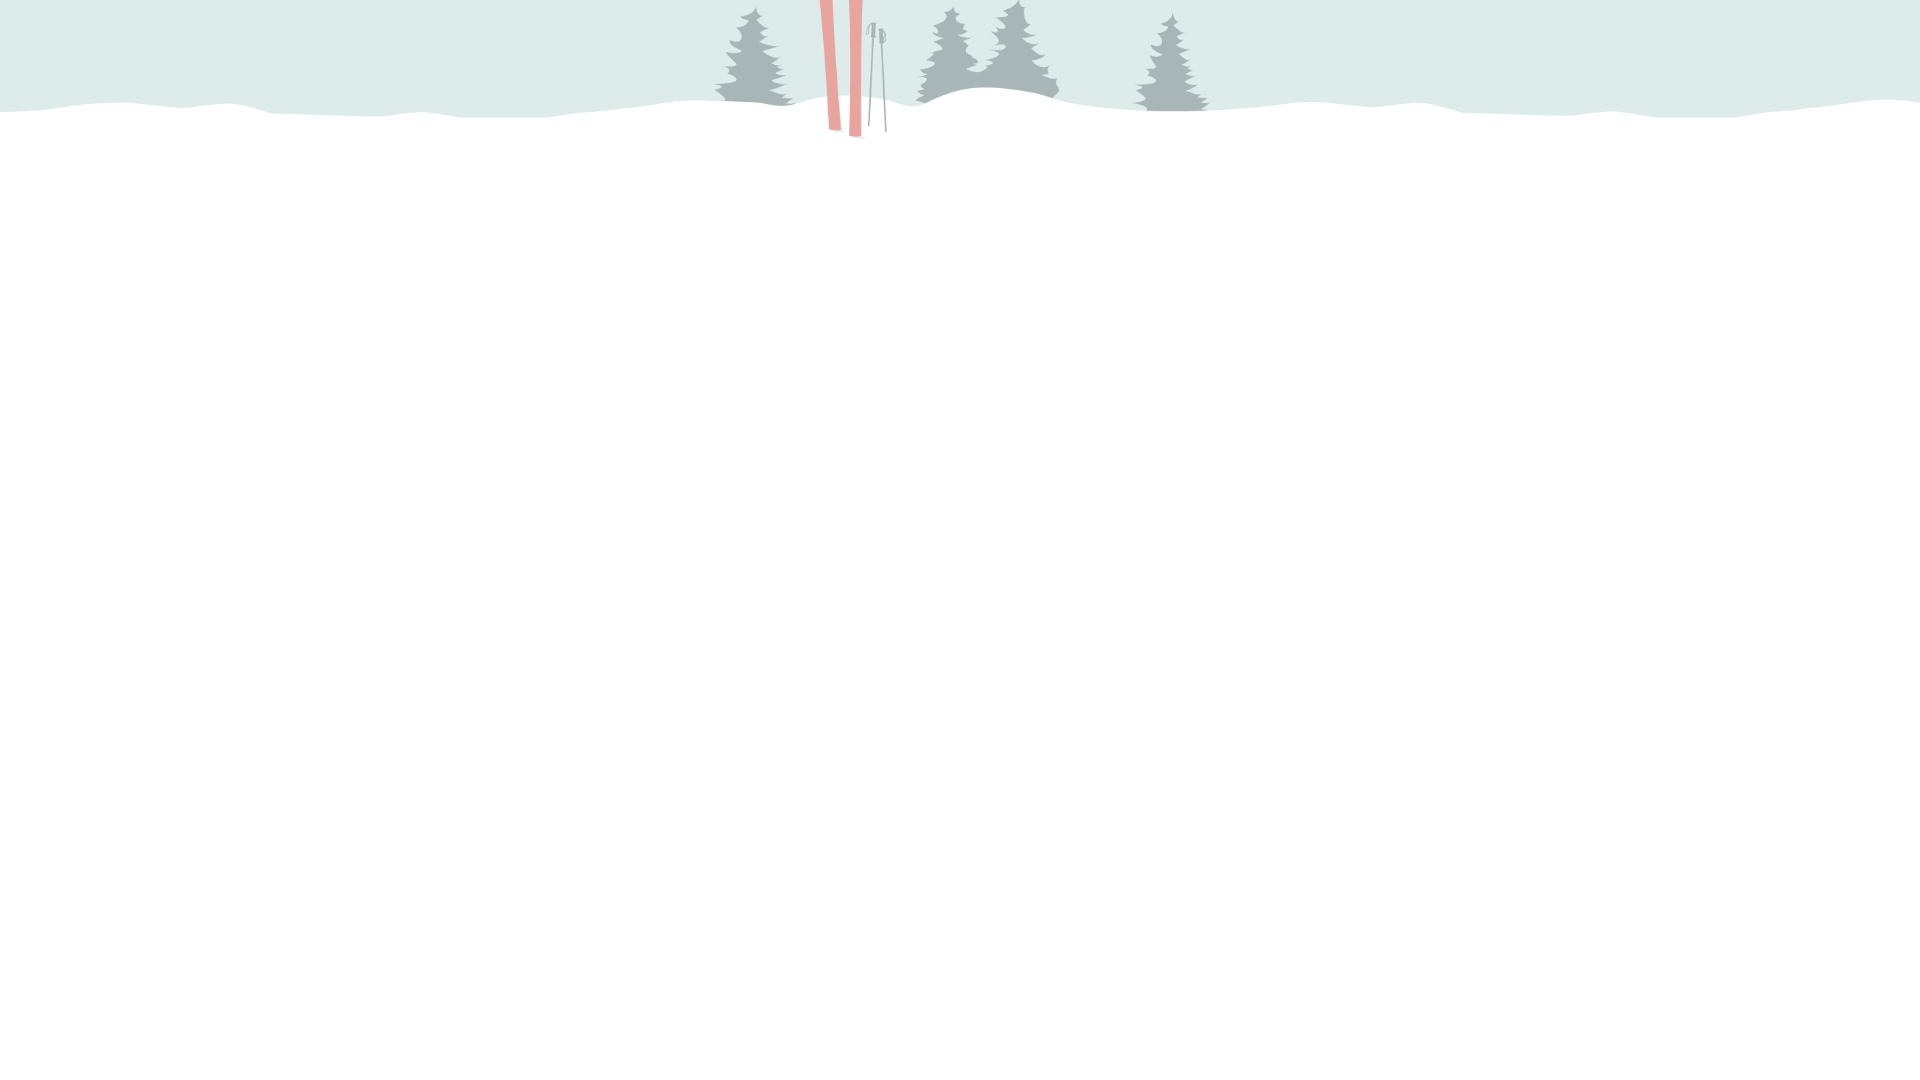
\includegraphics[width=\paperwidth,height=\paperheight]{bgbg.png}%
}

\title{Sensitivity conjecture}
\subtitle{\textellipsis{}or a \texorpdfstring{$1$}{1}-page proof of an \texorpdfstring{$\approx30$}{approx. 30} y.o. problem}
\author{Svyatoslav Gryaznov}
\institute{PDMI RAS}
\date{December 22, 2020}

\DeclareMathOperator{\s}{s}
\DeclareMathOperator{\bs}{bs}
\DeclareMathOperator{\degr}{deg}

\newcommand{\MM}{\widetilde{M}}
\newcommand{\RP}{\mathrm{RP}}
\newcommand{\AlgA}{\mathcal{A}}
\renewcommand{\Vec}[1]{\overline{#1}}

\newcommand{\Q}{{\{0,1\}}}

\begin{document}

\frame{\titlepage}

%\centering

\begin{frame}[t]{Sensitivity}
Let $f \colon \Q^n \to \Q$ be a Boolean function.

\begin{overprint}
\onslide<1>
\vspace{0.3in}
\begin{columns}[T]
\begin{column}{0.4\textwidth}
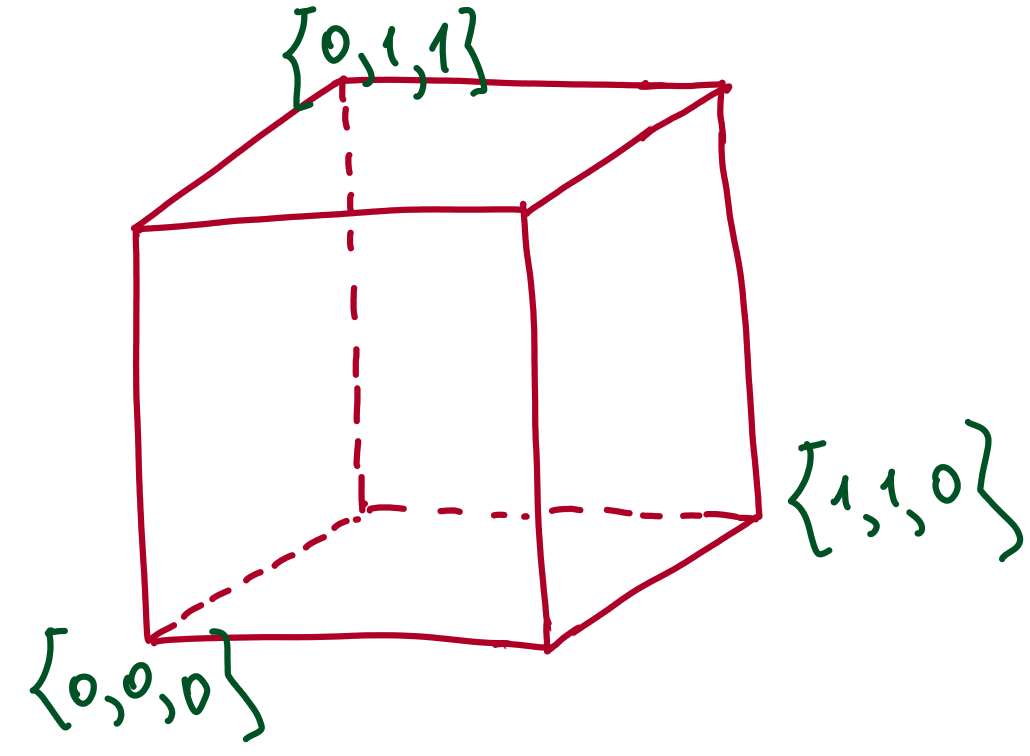
\includegraphics[width=1.4\textwidth]{cube.png}
\end{column}
\begin{column}{0.6\textwidth}
Is it \enquote{hard} to flip its value?
\begin{itemize}
    \item For a \emph{fixed} input:
    
    Can we change it by flipping only one bit?
    \item In the worst case?
\end{itemize}
\end{column}
\end{columns}
\onslide<2>
\begin{picture}(0,0)(-235, 25)
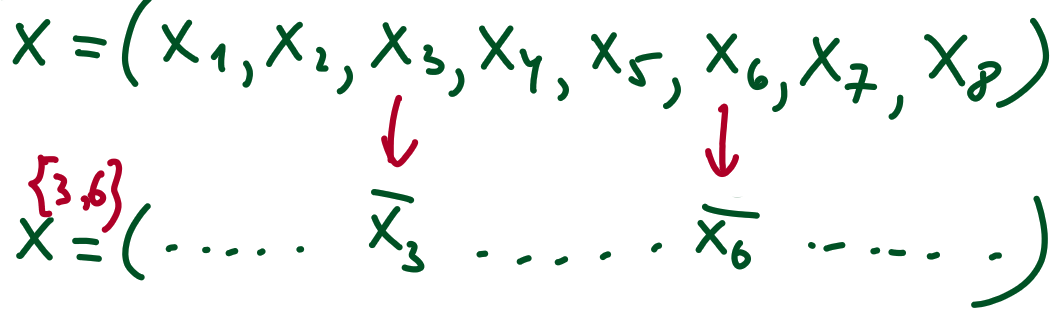
\includegraphics[scale=0.7]{sens.png}
\end{picture}%
For $x \in Q$ let $x^J$ be a vector with all $x_j$ flipped.
\vspace{0.25in}

\begin{itemize}
    \item For a fixed input $x \in Q^n$:
    \begin{align*}
        \s(f, x) = \max \left\{ |J| \;\middle|\; J \subseteq [n]: \forall i \in J.\; f(x) \neq f(x^{\{i\}}) \right\}
    \end{align*}
    
    \item In the worst case: $\s(f) = \max\limits_{x \in Q^n} \s(f, x)$
\end{itemize}
\end{overprint}
\end{frame}

\begin{frame}{Block sensitivity}
    \centering
    What if we can flip not only one bit, but a block of bits?
\end{frame}

\begin{frame}[t]{Block sensitivity}
Let $f \colon \Q^n \to \Q$ be a Boolean function.

\begin{picture}(0,0)(-235, 25)
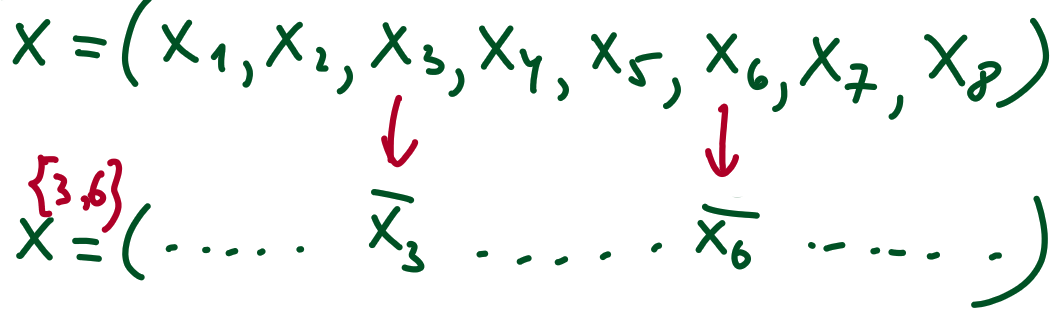
\includegraphics[scale=0.7]{sens.png}
\end{picture}%
For $x \in Q$ let $x^J$ be a vector with all $x_j$ flipped.
\vspace{0.25in}

\begin{itemize}
    \item For a fixed input $x \in Q^n$:
    \begin{align*}
        \bs(f, x) = \max \left\{ k \;\middle|\; B_1 \sqcup B_2 \sqcup \ldots \sqcup B_k \subseteq [n]: \forall i \in [k].\; f(x) \neq f(x^{B_k}) \right\}
    \end{align*}
    
    \item In the worst case: $\bs(f) = \max\limits_{x \in Q^n} \bs(f, x)$
    \begin{figure}
        \centering
        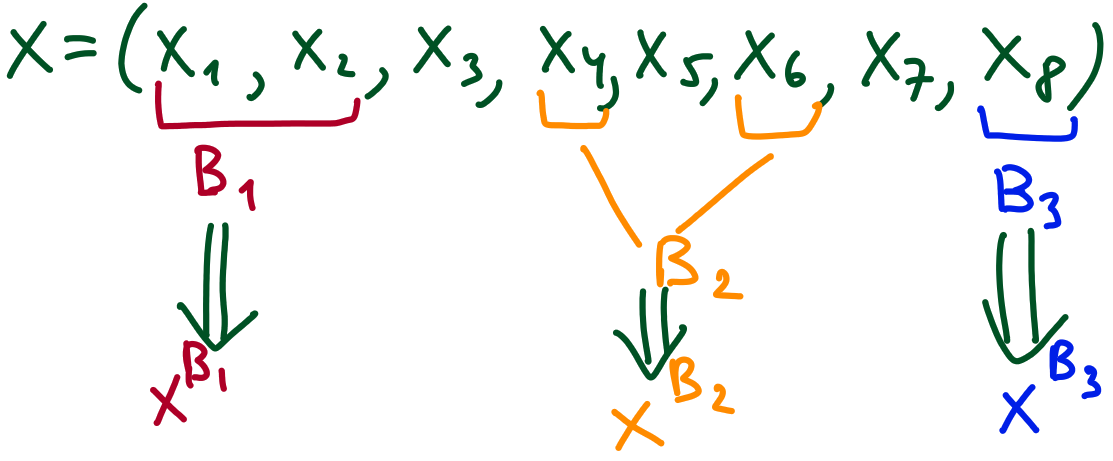
\includegraphics[scale=0.8]{bsens.png}
    \end{figure}
\end{itemize}
\end{frame}

\begin{frame}{Block sensitivity}
    \centering
    How are they related?
    \vspace{0.2in}
    
    \onslide<2->
    \begin{exampleblock}{}
        Obviously, $\s(f) \leq \bs(f)$.
    \end{exampleblock}
    \vspace{0.1in}
    \begin{overprint}
    \onslide<2>
    %\begin{picture}(0,0)(100, 95)
    %    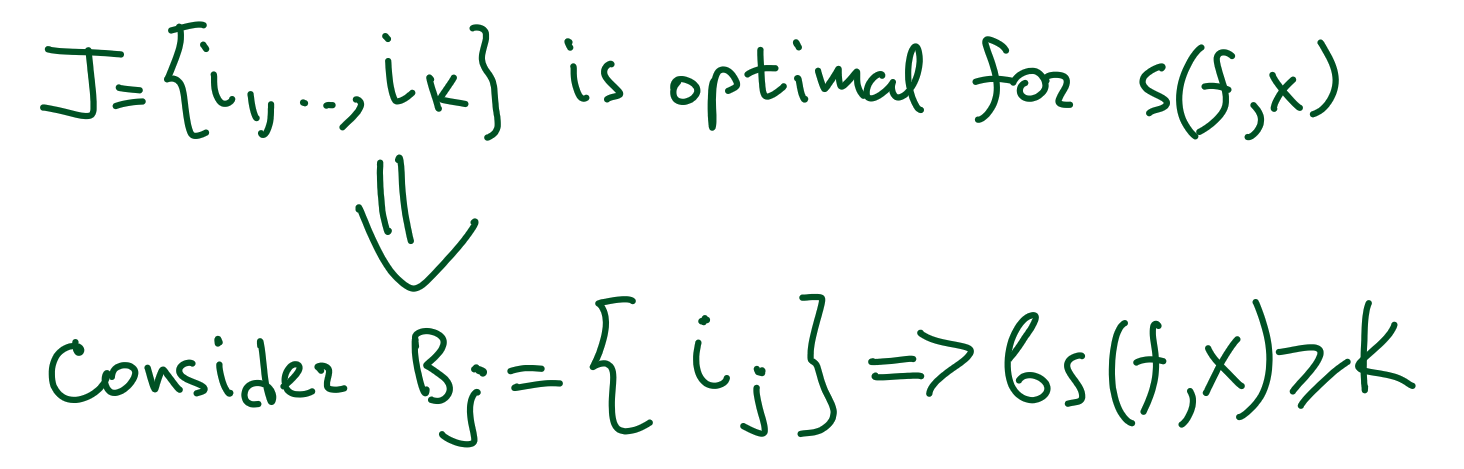
\includegraphics{s_bs.png}
    %\end{picture}}%
    \begin{figure}
        \centering
        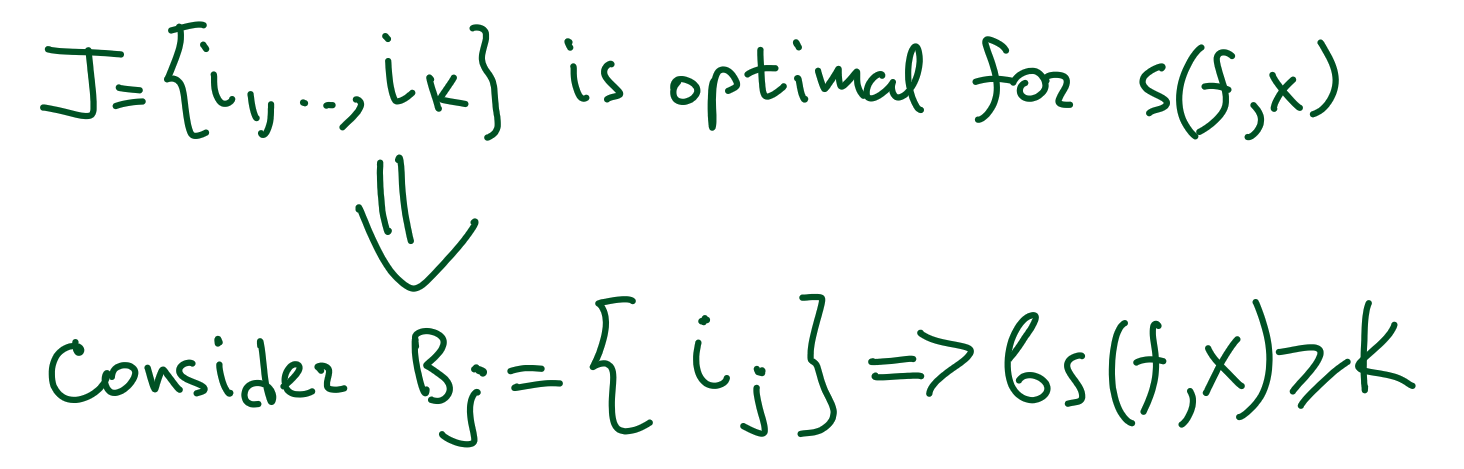
\includegraphics[scale=0.9]{s_bs.png}
    \end{figure}
    \onslide<3->
    \begin{block}{Sensitivity Conjecture [Nisan, Szegedy] (now Theorem [Huang])}
        \centering%
        \begin{equation*}
            \bs(f) \leq {\s(f)}^C \text{, for a fixed constant $C$ \geq 1}
        \end{equation*}
        (It holds for $C=4$)
        \linebreak
    \end{block}
    \end{overprint}
\end{frame}

\begin{frame}{Why?}
    Low-sensitivity (or \enquote{smooth}) functions:
    \begin{itemize}
        \item<2-> (\textbf{Computational}) are easy to compute even in the simplest models (like decision trees).
        \item<3-> (\textbf{Algebraical}) have low degree as real polynomials.
        \item<4-> Combinatorial applications.
        \item<4-> Randomized and quantum query complexity.
        \item<4-> Certificate complexity.
        \item<4-> \textellipsis{}
    \end{itemize}
\end{frame}

\begin{frame}{Computational application: Decision trees}
    \begin{equation*}
        f\colon \Q^n \to \Q
    \end{equation*}
    \begin{columns}[T]
    \begin{column}{0.55\textwidth}%
    \vspace{-0.42in}%
    \begin{figure}
        \centering
        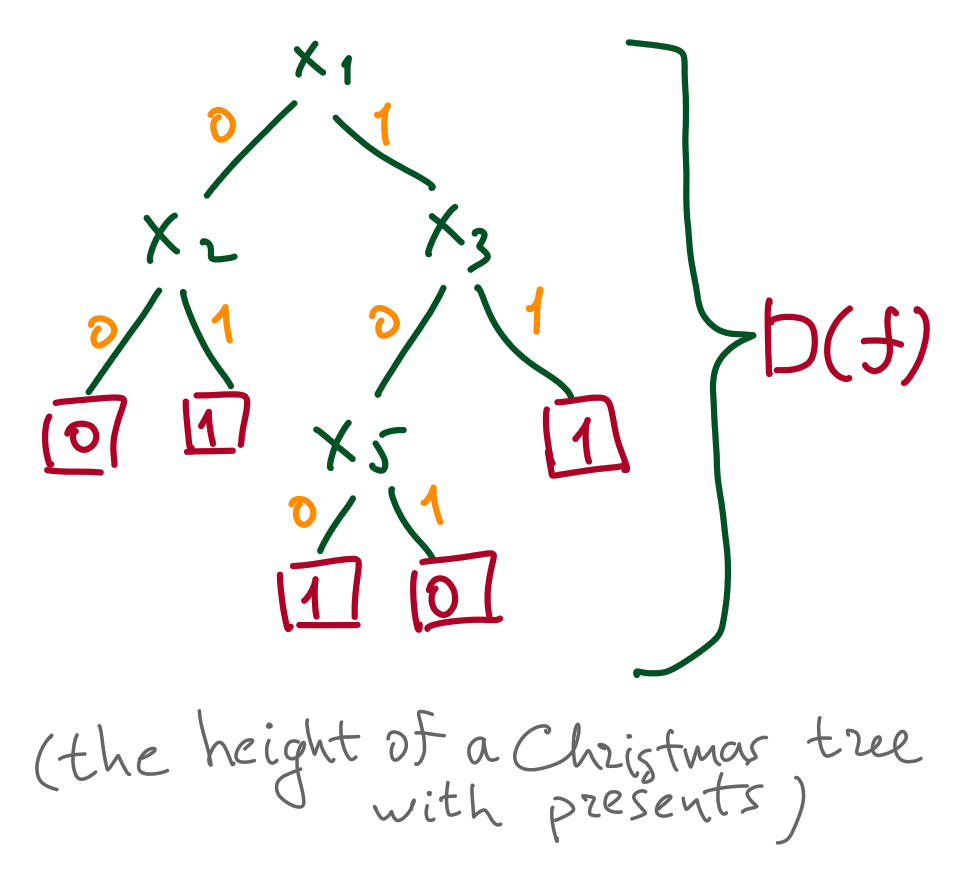
\includegraphics[scale=0.98]{decision_tree.png}
    \end{figure}
    \end{column}
    \begin{column}{0.45\textwidth}%
    \vspace{0.5in}%
    \begin{block}{Relation with decision trees}
    \begin{equation*}
        \bs(f) \le D(f) \le {\bs(f)}^3
    \end{equation*}
    \end{block}
    \end{column}
    \end{columns}
\end{frame}

\begin{frame}{Algebraic application}
    Polynomial $p\colon \mathbb{R}^n \to \mathbb{R}$ represents $f$ if
    \begin{equation*}
        \text{For all } x \in \Q^n.\; p(x) = f(x).
    \end{equation*}
    The degree $\degr(f)$ of $f$ is the degree of a unique multilinear $p$ that represents $f$.
    \begin{block}{Relation with $\degr{f}$}
    \begin{equation*}
        \sqrt{\bs(f)} \le \degr(f) \le {\bs(f)}^3
    \end{equation*}
    \end{block}
\end{frame}

\begin{frame}{Supplementary Theorem}
    Let $f \colon \Q^n \to \Q$ be a Boolean function.
    \vspace{0.3in}
    
    \begin{columns}[T]
    \begin{column}{0.4\textwidth}
    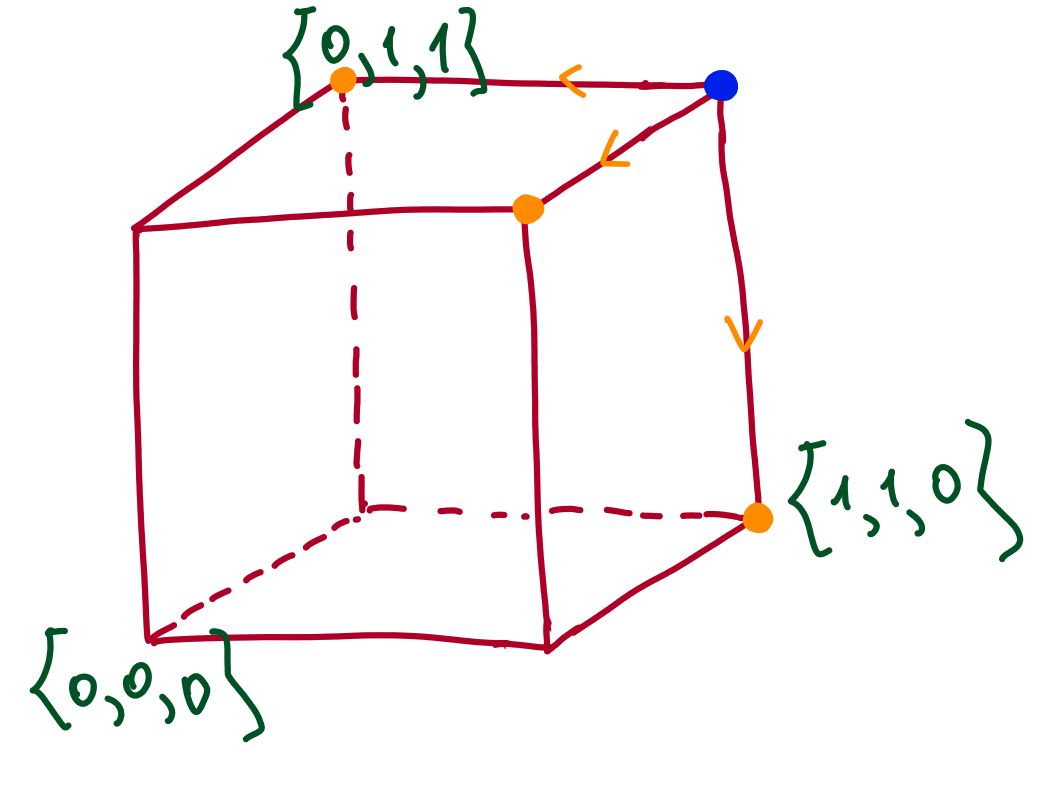
\includegraphics[width=1.4\textwidth]{cube_neighbors.png}
    \end{column}
    \begin{column}{0.6\textwidth}
    It is enough to prove:
    \begin{block}{Theorem: vertex with large degree}
    Any set $H$ of $2^{n-1}+1$ vertices of $\Q^n$ contains a vertex with degree $\geq \sqrt{n}$.
    \end{block}
    \end{column}
    \end{columns}
\end{frame}

\begin{frame}{What we need}
    \begin{block}{Folklore}
         The linear system of $m$ equations and $m+1$ variables has a non-trivial solution.
    \end{block}
\end{frame}

\begin{frame}{Proof (a simplification by Fedya Petrov)}
    \begin{columns}
    \begin{column}{0.7\textwidth}
    \textbf{Not-identically-zero} function $f\colon \Q^n \to \mathbb{R}$:
    \begin{itemize}
        \item $f(x), x \in \Q^n$ are variables.
        \item $f$ vanishes outside $H$: $2^{n-1}-1$ equations.
        \item $f$ satisfies \textbf{some} other $2^{n-1}$ equations.
    \end{itemize}
    Exists by the theorem above.
    \end{column}
    \begin{column}{0.3\textwidth}
    \begin{picture}(0, 0)(80, 110)
    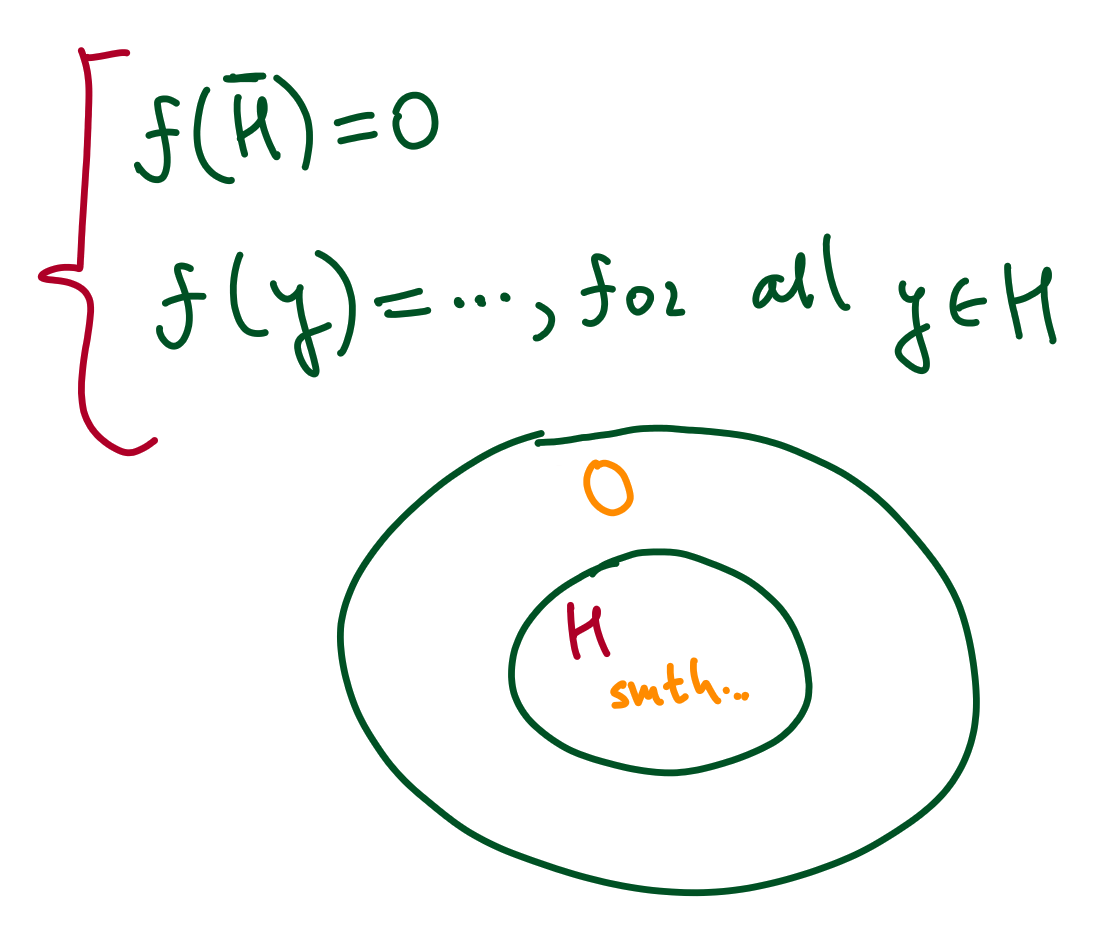
\includegraphics[scale=0.75]{good_f.png}
    \end{picture}
    \end{column}
    \end{columns}
\end{frame}

\begin{frame}{Proof: Weight function}
For $x = (x_1, \ldots, x_k)$ define
\begin{equation*}
    w_i(x) = {(-1)}^{x_1 + \ldots + x_{i-1}}.
\end{equation*}
Clearly:
\begin{equation*}
    w_i(x) = w_i(x^i).
\end{equation*}
Also:
\begin{equation*}
    w_i(x) w_j(x) w_i(x^j) w_j(x^i) = -1 \text{ for } i \neq j.
\end{equation*}
\end{frame}

\begin{frame}{Proof: Relations}
    \begin{align*}
        \sqrt{n} \cdot f(y) = \sum\limits_{i=1}^n w_i(y) f(y^i), \text{ for all } y \in \Q^n.
    \end{align*}
    They're linearly dependent:
    
    For $y=(x_1, \ldots, x_{n-1}, 0) = x0$:
    \begin{align*}
        \sqrt{n} \cdot f(x0) = f(x1) + \sum\limits_{i=1}^{n-1} w_i(x) f(x^i0), \text{ for all } y \in \Q^n, \\
        \sqrt{n} \cdot f(x1) = f(x0) - \sum\limits_{i=1}^{n-1} w_i(x) f(x^i1), \text{ for all } y \in \Q^n.
    \end{align*}
    
    Now substitute the former into the latter.
\end{frame}

\begin{frame}{Proof: QED}
    Choose $y \in \Q^n$ s.t. $\left| f(y) \right|$ is maximal. From
    \begin{align*}
        \sqrt{n} \cdot f(y) = \sum\limits_{i=1}^n w_i(y) f(y^i), \text{ for all } y \in \Q^n.
    \end{align*}
    it follows that for at least $\sqrt{n}$ elements $f(y^i) \neq 0$, hence they are in $H$.
    
    \begin{picture}(0,0)(-335, 20)
    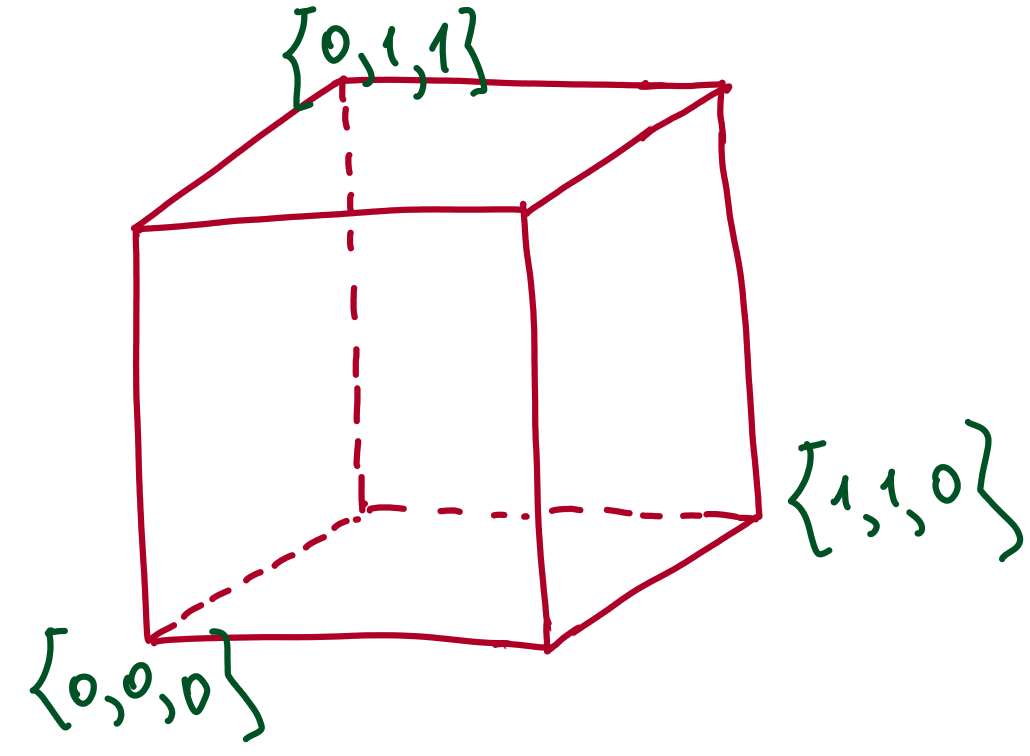
\includegraphics[scale=0.2]{cube.png}
    \end{picture}%
\end{frame}

\begin{frame}{Proof: Motivation}
    There is only $2^{n-1}$ linearly independent equations since the operator
    \begin{equation*}
        f(y) \mapsto \sum\limits_{i=1}^n w_i(y) \cdot f(y^i)
    \end{equation*}
    has an eigensubspace of dimension $2^{n-1}$ for the eigenvalue $\sqrt{n}$.
\end{frame}

\begin{frame}{Possibly Part 2}
    \begin{itemize}
        \item<1-> Why we defined such an operator?
        \item<2-> It can be explained using expander graphs.
    \end{itemize}
\end{frame}

% Consider matrices $A_n$ of size $2^n$:
% \begin{equation*}
% \begin{array}{cc}
%     A_0 = \begin{pmatrix}
%     0
%     \end{pmatrix};\quad &
%     A_n = \begin{pmatrix}
%     A_{n-1} & I_{2^n-1} \\
%     I_{2^n-1} & -A_{n-1}
%     \end{pmatrix}, \text{ for } n > 0.
% \end{array}
% \end{equation*}
% By induction $A_n^2 = nI_{2_n}$ for all $n \geq 0$.

% \begin{frame}{Graphs}
% \begin{columns}
% \begin{column}{0.3\textwidth}
% \includegraphics[width=1.5\textwidth]{graph.png}
% \end{column}
% \begin{column}{0.7\textwidth}  %%<--- here
% \begin{gather*}
% G = (V, E) \\
% E \subseteq V \times V \\
% \text{unordered: } (u,v) \in E \iff (v,u) \in E \\
% \text{regular: } \deg(v) = d \\
% \text{connected}
% \end{gather*}
% \end{column}
% \end{columns}
% \end{frame}

\end{document}